\chapter{Standard Proposal: Guidance on the Development of PX Questionnaires}
\label{ch:questionnaire}

% Introduction (Explain and contextualise objective)
% 
One of the most employed \ac{PX} evaluation methods is using questionnaires. A questionnaire allows collecting self-reported data from players before, during or after interacting with a game. Although there are some standardised \ac{PX} questionnaires \autocite{denisova_convergence_2016,VandenAbeele2016,Calvillo-Gamez2015,Brockmyer2009,Poels2008,DeKort2007,Vorderer2004}, the most common approach is to develop ad-hoc questionnaires to evaluate \ac{PX} \autocite{Yanez-Gomez2017}. In the case of \acp{PREG}, we identified constraints that can represent challenges when evaluating \ac{PX} in \autoref{ch:characterising}. Existing standardised questionnaires may be useful to evaluate aspects such as enjoyment, immersion, presence and flow. However, evaluating \ac{PX} in \acp{PREG} may require developing questionnaires that address those constraints.

Nevertheless, there is no a standardised process to develop a questionnaire for \ac{PX} or even \ac{UX} evaluation. Existing questionnaires have been developed following different approaches. In this chapter, we present the design of a standard proposal to develop questionnaires to evaluate \ac{PX}. Our proposal is based on 22 documents that we reviewed to identify and integrate recommendations, guides and adopted practices for developing questionnaires. Also, we studied the current status of standardisation in the \ac{UX} field to identify how to develop a standard properly; i.e., following guidelines of a relevant standardisation organisation. Then, we integrated our findings into a standard process.

% -----------------------------------------------
\section{Standardisation} % Standardisation -----------------------------------------------
\label{sec:standardisation}
To the extent of the author's knowledge, a standard to develop questionnaires to evaluate \acp{PREG} is not defined. However, there are usability and \ac{UX} standards which are a relevant reference for the process of standardising \ac{PX}. Below, we present a review of \ac{UX} standards.

\textcite{Ran2015} present a summary of standards and standardisation organisations related to usability and \ac{UX} (See \autoref{fig:standardisation_orgs}). The most influential international organisations are \ac{ISO}, \ac{IEC} and \ac{ITU} \autocite{Ran2015}. While, \ac{CEN} and \ac{ETSI} are relevant European standardisation organisations.

\ac{ISO} formulated the \textit{ISO 9241} standards, which are considered general and broad and have had the highest impact \autocite{Ran2015}. The most relevant parts of this standard are \textit{ISO 9241:11} \autocite{iso9241:11} and \textit{ISO 9241:210} \autocite{iso9241:210}. The first one, guides users on the usability of hardware and software systems; and the second one, guides the design of human-centred interactive systems and introduces the concept of \ac{UX}.

Meanwhile, the TC 122 working group from \ac{CEN} organisation works on ergonomics standardisation for designing work systems and work environments. A list of standards published by this working group can be found at its website\footnote{\ac{CEN} TC 122 standards: \url{https://standards.cen.eu}}. The \ac{IEC} technical committee ISO/IEC JTC 1/SC 35 works on user interfaces standardisation for \ac{ICT}. A list of publications from this committee can be accessed from its website\footnote{ISO/IEC JTC 1/SC 35 publications: \url{http://www.iec.ch}}.

The other two organisations formulate \ac{UX} and usability standards in specific fields. First, \ac{ETSI} has formulated several standards in human factors and accessibility of \ac{ICT}, including fixed, mobile, radio, broadcast and internet technologies. These standards can be accessed at the organisation's website\footnote{\ac{ETSI} standards: \url{http://www.etsi.org/technologies-clusters/technologies/human-factors-accessibility}}. Meanwhile, \ac{ITU} and specifically the study group 12 works on standards for performance, \ac{QoE} and \ac{QoS} of next-generation networks\footnote{\ac{ITU} standards: \url{https://www.itu.int/en/ITU-T/studygroups/2017-2020/12/Pages/default.aspx}}.

\begin{figure}[htb]
\myfloatalign
{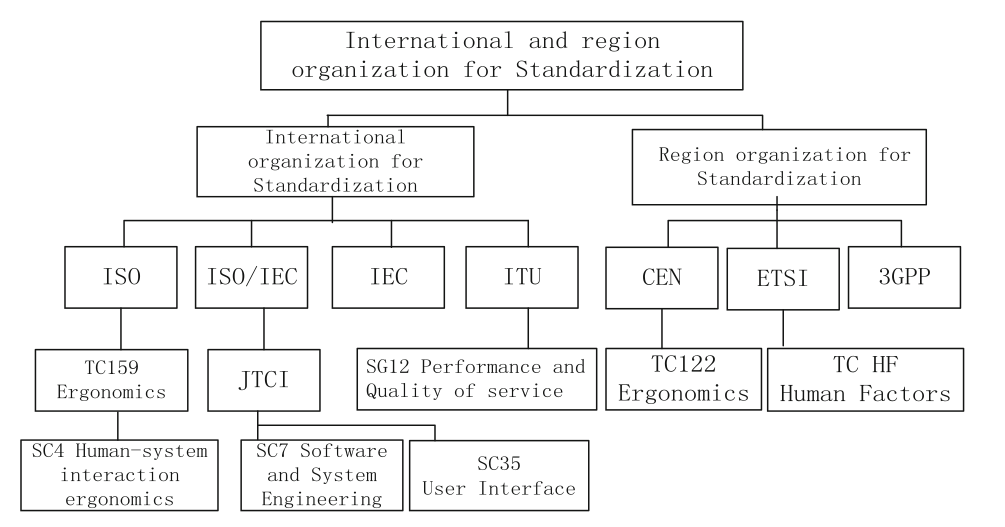
\includegraphics[width=\linewidth]{gfx/standard/standardisation_orgs}} \quad
\caption[Standardisation organisations related to usability and \ac{UX}]{Standardisation organisations related to usability and \ac{UX} \autocite{Ran2015}}\label{fig:standardisation_orgs}
\end{figure}

Most of these standards are not publicly available. From the above organisations only \ac{ETSI} provide copies of its standards directly at its website.

\subsection{ISO 9241:210}
As mentioned above, ISO 9241 Ergonomics of human-system interaction standards are the most relevant in the field of \ac{UX} \autocite{Ran2015}. From these standards, the ISO 9241:210 \autocite{iso9241:210} is of high relevance since it introduces the concept of \ac{UX}. According to this standard, \ac{UX} can be defined as "person's perceptions and responses resulting from the use and/or anticipated use of a product, system or service". The standard also mentions three notes about this definition. The first note highlights that \ac{UX} includes the experience before, during and after use. The second note explains that \ac{UX} also is affected by characteristics of the interactive system, the users internal and physical state and the context of use. The third note explains that \ac{UX} can be considered and evaluated as usability when it is interpreted from the perspective of users' personal goals.

Additionally to \ac{UX}, this standard presents other definitions including accessibility, context of use, usability, usability attributes, interactive system and human centred design. Moreover, it describes some benefits of adopting human-centred design; e.g., \ac{UX} improving, productivity increasing, ease of understanding, cost reduce among others.

The standard also describes six principles of human-centred design:

\begin{enumerate}
    \item the design is based upon an explicit understanding of users, tasks and environments
    \item users are involved throughout design and development
    \item the design is driven and refined by user-centred evaluation
    \item the process is iterative
    \item the design addresses the whole \ac{UX}
    \item the design team includes multidisciplinary skills and perspectives
\end{enumerate}

The third principle indicates that evaluation must be carried out to gather feedback from users. This evaluation may reduce the risk of producing a system which does not meet user needs. Other, principles may also apply to evaluation; i.e., users involvement, whole \ac{UX}, iterative process and multidisciplinary skills are also desirable for \ac{UX} evaluation.

Furthermore, the document details the activities of the human-centred design process, which are presented in \autoref{tab:huma_centred_activities} and detailed in \autocite{iso25060}.

\begin{table}[htb]
\caption[Activities of the human-centred design process]{Activities of the human-centred design process}
\label{tab:huma_centred_activities}
\myfloatalign
\resizebox{\linewidth}{!}{
\begin{tabular}{lp{5.5cm}}
\toprule
%----------------------
\spacedlowsmallcaps{Activities} 
& \spacedlowsmallcaps{Outputs}
\\ \midrule
%----------------------
Understand and specify the context of use
&
Context of use description
\\
\midrule
%----------------------
\multirow{3}{*}{Specify the user requirements}
&
Context of use specification
\\&
User needs description
\\&
User requirements specification
\\\midrule
%----------------------
\multirow{3}{5.5cm}{Produce design solutions to meet these requirements}
&
User interaction specification
\\&
User interface specification
\\&
Implemented user interface
\\\midrule
%----------------------
\multirow{3}{5.5cm}{Evaluate the designs against requirements}
&
Evaluation results
\\&
Conformance test results
\\&
Long-term monitoring results
\\\midrule
%----------------------
\bottomrule
\end{tabular}}
\end{table}

The last human centred-design activity is \textit{Evaluating the design}. According to this standard, evaluators should evaluate a design concept from the user's perspective. That would allow evaluators to gain a better understanding of users' needs is gained. However, the direct participation of users is not completely necessary; i.e, evaluators can employ inspection-based evaluation. A human-centred evaluation allows collecting new information about users, gathering the strengths and weaknesses of the design solution, assessing user requirements achievement and establishing baselines to compare different designs.

According to the standard, a user-centred evaluation should involve allocating resources for early and late evaluation, planning, carrying sufficient testing out, analysing results, proposing solutions and communicating those solutions to the design team. Evaluations can be carried out along the whole project life cycle.

The standard presents two approaches for user-centred evaluation: 

\begin{itemize}
    \item \emph{User-based evaluation}: requires the participation of users. At early stages, it allows testing design concepts against the real world. Also, evaluators can collect feedback about the acceptability of a design.
    At later stages, evaluators can assess the achievement of usability objectives in the context of use.
    \item \emph{Inspection-based evaluation}: involves the participation of usability experts who play the role of users to evaluate the system. Evaluators use their knowledge, guidelines, heuristics and standards among others. This kind of evaluation is cost-effective; however, it relies on the evaluators' skills and knowledge.
\end{itemize}

User-centred evaluation methods and guidance on how and when to use them are presented in \autocite{iso16982}.

%-----------------------------------
\section{Materials and methods} % Materials -----------------------------------
\label{sec:mats_mets_sta}

We conducted a literature review to identify recommendations and current practices in the development of questionnaires. We reviewed 21 documents, 14 documents reported the development of \ac{UX} or \ac{PX} questionnaires and the remaining 7 corresponded to guides for developing and composing questionnaires (See \autoref{tab:rev_docs_sta}). We identified the stages, activities, methods and best practices employed or suggested in each document. Then, we classified and grouped findings to compose a comprehensive process to develop questionnaires for \ac{PX} evaluation. The conducted process is illustrated in \autoref{fig:methods_sta}.

\begin{table}[htp]
\caption{Reviewed documents to develop the standard proposal}
\label{tab:rev_docs_sta}
\myfloatalign
\resizebox{\linewidth}{!}{
\begin{tabular}{p{3cm}l}
\toprule
%----------------------
\spacedlowsmallcaps{Type} 
& \spacedlowsmallcaps{Document Title}
\\ 
\midrule
%----------------------
\multirow{7}{3cm}{\ac{PX} Questionnaire} &
Assessing the Core Elements of the Gaming Experience \autocite{Calvillo-Gamez2015}
\\
%\cline{2-2}
%----------------------
& FUGA-the fun of gaming: measuring the human experience of media enjoyment \autocite{Poels2008}
\\
%\cline{2-2}
%----------------------
& The development of the Game Engagement Questionnaire: A measure of engagement in video game-playing \autocite{Brockmyer2009}
\\
%\cline{2-2}
%----------------------
& MEC spatial presence questionnaire (MEC-SPQ): Short documentation and instructions for application \autocite{Vorderer2004}
\\
%\cline{2-2}
%----------------------
& Digital games as social presence technology: Development of the Social Presence in Gaming Questionnaire (SPGQ) \autocite{DeKort2007}
\\
%\cline{2-2}
%----------------------
& Rapid assessment of game experiences in public settings \autocite{Moser2012}
\\
%\cline{2-2}
%----------------------
& The convergence of player experience questionnaires \autocite{Denisova2016}
\\
\midrule
%----------------------
\multirow{2}{3cm}{\ac{PX} Scale} &
EGameFlow: A scale to measure learners’ enjoyment of e-learning games \autocite{Fu2009}
\\
%\cline{2-2}
%----------------------
& Design and preliminary validation of the Player Experience Inventory \autocite{VandenAbeele2016}
\\
\midrule
%----------------------
\multirow{2}{3cm}{\ac{UX} Questionnaire} &
Construction and evaluation of a User Experience Questionnaire \autocite{Laugwitz2008}
\\
%\cline{2-2}
%----------------------
& AttrakDiff: Ein Fragebogen zur Messung wahrgenommener hedonischer und pragmatischer Qualität \autocite{Hassenzahl2003}
\\
\midrule
%----------------------
\multirow{2}{3cm}{Usability Questionnaire} &
Measuring usability with the use questionnaire \autocite{lund2001measuring}
\\
%\cline{2-2}
%----------------------
& Development of an instrument measuring user satisfaction of the Human-computer Interface \autocite{Chin1988}
\\
\midrule
%----------------------
Usability scale
&
SUS-A quick and dirty usability scale \autocite{Brooke1996}
\\
\midrule
%----------------------
\multirow{7}{3cm}{Guide} &
Administering, analysing, and reporting your questionnaire \autocite{Boynton2004}
\\
%\cline{2-2}
%----------------------
& Reaching beyond the white middle classes \autocite{Boynton2004b}
\\
%\cline{2-2}
%----------------------
& Selecting, designing, and developing your questionnaire \autocite{Boynton2004c}
\\
%\cline{2-2}
%----------------------
& A step-by-step guide to developing effective questionnaires and survey procedures for program evaluation \& research \autocite{Diem}
\\
%\cline{2-2}
%----------------------
& Questionnaire design \autocite{Crawford1997}
\\
%\cline{2-2}
%----------------------
& Tips for developing and testing questionnaires/instruments \autocite{Radhakrishna2007}
\\
%\cline{2-2}
%----------------------
& Question and questionnaire design \autocite{Krosnick2009}
\\
\midrule
%----------------------
\bottomrule
\end{tabular}}
\end{table}

\begin{figure}[htb]
\myfloatalign
{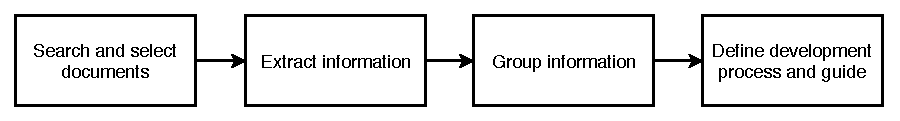
\includegraphics[width=\linewidth]{gfx/standard/MethodStad}} \quad
\caption{Process conducted to develop the questionnaires standard proposal}\label{fig:methods_sta}
\end{figure}

The standard proposal was composed following the principles and rules for the structure and drafting of documents by \ac{ISO}, \ac{IEC} \autocite{ISO2016}.

%-----------------------------------
\section{Standard Proposal: Guidance on Questionnaires Development} % Results -----------------------------------
% Requirement: shall, shall not. 
% Recommendation: should, should not
% Permission: may, need not
% Possibility and capability: can, cannot
% External constraint Verbal: must

\label{sec:sta_proposal}

\subsection{Introduction}
A questionnaire is a data collection method that allows gathering information from people. A reliable and valid questionnaire can be used over time by different interviewers or researchers, involving different samples of the target audience. As a consequence, one can compare the results of different studies objectively.

This document aims to provide guidance on how to develop a valid and reliable questionnaire to those responsible for evaluating \ac{PX} aspects using questionnaires.

\subsection{Scope}

This document specifies a process for developing valid and reliable questionnaires for evaluating \ac{PX} aspects. Also, it includes a guide for formulating questions. It is intended to be used by those responsible for developing questionnaires to evaluate \ac{PX} aspects collecting information from a specific audience. The process encompasses the preparation, design and pre-testing of a questionnaire. It does not provide detailed coverage of specific techniques and methods associated questionnaire development activities.

Presentation, format, layout and styles of questionnaires are outside the scope of this document.

\subsection{Normative references}
There are no normative references in this document.

\subsection{Terms and definitions}
For the purposes of this document, the following terms and definitions apply.

\subsubsection{Questionnaire}
A data collection method that helps gather information about knowledge, attitudes, opinions, behaviours, facts and other information \cite{Radhakrishna2007}.

\subsubsection{Standardised questionnaire}
A questionnaire that is written and administered precisely. That is, all respondents are asked the same questions, and their responses are registered uniformly \cite{Boynton2004c}.

\subsubsection{Researcher}
A person who develops a questionnaire.

\subsubsection{Interviewer}
A person who administers a questionnaire.

\subsubsection{Respondent}
A person who answers a questionnaire.

\subsubsection{Valid questionnaire}
A questionnaire that measures what it is intended to measure \cite{Boynton2004c}.

\subsubsection{Reliable questionnaire}
A questionnaire that produces consistent results for repeated samples and when administered by different interviewers \cite{Boynton2004c}.

\subsubsection{Closed question}
A question that requires respondents to select an answer from a set of choices \cite{Krosnick2009}.

\subsubsection{Screening question}
A question that may have follow-up questions depending on how respondents answer it \cite{Krosnick2009}.

\subsection{Symbols and abbreviated terms}
\begin{acronym}[UML]
\acro{PX}{Player Experience}
\acro{UX}{User Experience}
\acro{HCI}{Human Computer Interaction}
\acro{AI}{Artificial Intelligence}
\end{acronym}

\subsection{Questionnaire development process}

\autoref{fig_quesDevProcess} presents the process of questionnaire development. It comprises three main activities and involves three decisions. Throughout the process, researchers will develop or select a valid and reliable questionnaire for evaluating one or more \ac{PX} aspects. The process is detailed below.

\begin{figure}[htb]
\myfloatalign
{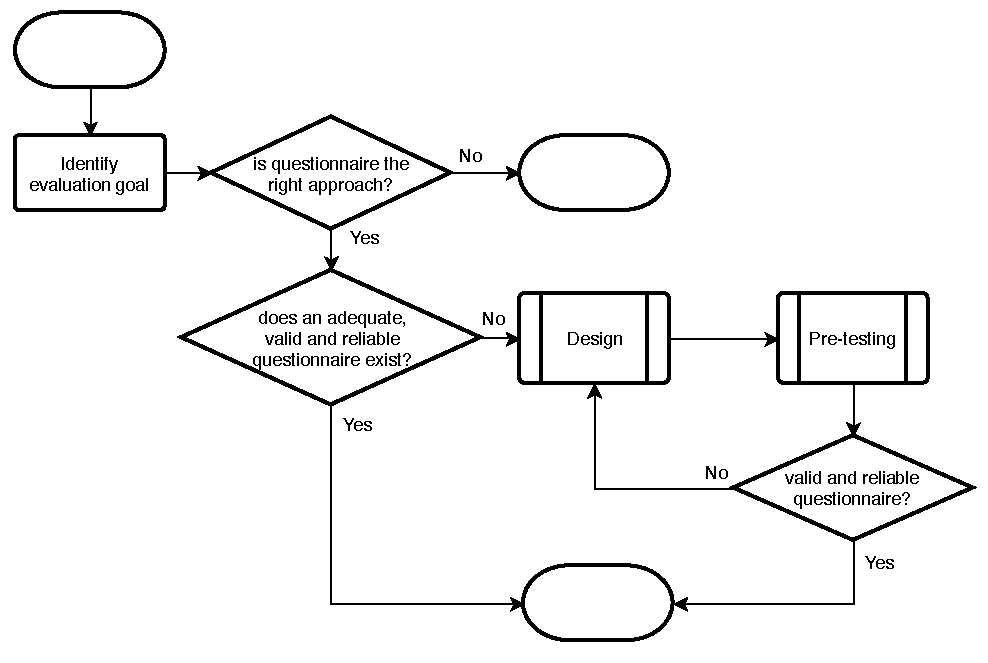
\includegraphics[width=0.9\linewidth]{gfx/standard/quesDevProcess}} \quad
\caption{Questionnaire development process}\label{fig_quesDevProcess}
\end{figure}

\subsubsection{Identify evaluation goal}
In this stage, researchers determine the information they need to know and the reasons to know it. This may result in the identification of an \emph{evaluation goal} \cite{Diem,Radhakrishna2007,Crawford1997}. Nevertheless, defining an evaluation is not straightforward since it involves exploratory research. That includes consulting experts or collecting data from people directly related to the problem itself; e.g. by performing a focus group, reviewing literature \cite{Crawford1997}.

\subsubsection{Is questionnaire the right approach?}
Researchers determine whether using a questionnaire is the right approach to achieve the evaluation goal \cite{Boynton2004c}. Depending on the goal, other data collection methods may be more appropriate than questionnaires; e.g. observation, video recording, interview and existing data analysis among others. A multi-method approach may also be convenient \cite{Boynton2004c,Krosnick2009}, in such a case, researchers should define a more specific goal for the questionnaire.

If a questionnaire is not appropriate to meet the evaluation goal, the development process finishes since no questionnaire is to be selected or designed.

\subsubsection{Does an adequate, valid and reliable questionnaire exists?}
Researchers determine whether they can employ an existing questionnaire instead of designing a new one \cite{Boynton2004c}. If researchers have conducted an exploratory research in the first stage, they might have an initial idea of how similar studies were carried out and what instruments were employed. Otherwise, they should conduct an additional exploration to identify existing questionnaires, which could be employed to achieve research objectives. If any questionnaire is available, researchers should identify whether it is reliable and valid. Note they shall prefer standardised questionnaires over other alternatives \cite{Boynton2004c}.

If researchers identify an appropriate, valid and reliable questionnaire; they can use it and this process finishes. Otherwise, researchers should continue with the design stage.

\subsubsection{Design}
Researchers decide on questions, wording, format and layout among others. The main output of this stage is a version of the questionnaire and accompanying documents. This step comprises a whole sub-process, which is described in \autoref{sec:ques_design}.

\subsubsection{Pre-testing}
Researchers test the questionnaire they designed during the last stage. Pre-testing should be planned, and the data should be collected, processed, analysed and reported. Researchers should establish the validity and reliability of the designed questionnaire. This step comprises a whole process, which is described in \autoref{sec:ques_pretesting}.

\subsubsection{Validity and reliability check}
Researchers determine whether the designed questionnaire is valid and reliable enough. If so, the process is finished successfully. Otherwise, researches should return to the design stage and iterate until they achieve the desired reliability and validity.

\subsection{Questionnaire design}
\label{sec:ques_design}
Designing a questionnaire is a respondent centred process. It requires researchers to determine the aspects to be studied and define the target respondents. Then, researchers shall produce questions that allow studying those aspects. Those questions shall be understood and answered accurately by target respondents. To achieve that, researchers should take care of wording, format, number and order of questions. \autoref{fig_quesDesignProcess} shows an overview of the process and further details are provided below.

\begin{figure}[htb]
\myfloatalign
{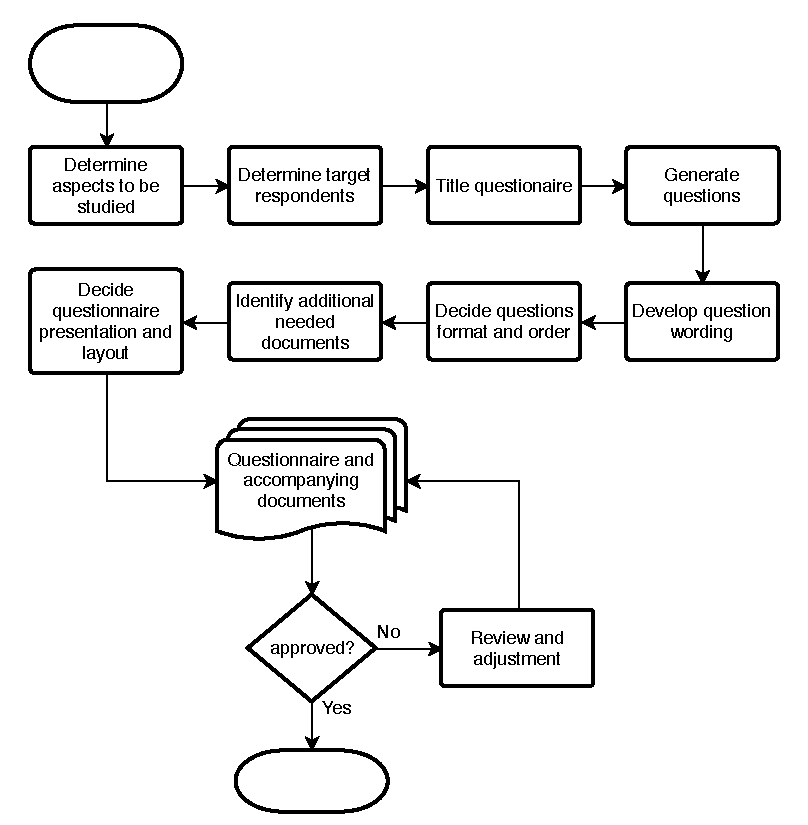
\includegraphics[width=0.9\linewidth]{gfx/standard/quesDesignProcess}} \quad
\caption[Questionnaire design process]{Questionnaire design process}\label{fig_quesDesignProcess}
\end{figure}

\subsubsection{Determine aspects to be studied} 
Researchers shall define which \ac{PX} aspects they will study to achieve the defined evaluation goal. Examples of \ac{PX} aspects include motivation, effectiveness, ease of use, attractiveness.

\subsubsection{Determine target respondents}
Researches shall define the appropriate population to be asked. This step also includes identifying characteristics of the target respondents that should be considered during the design process, e.g., age, education level, familiarity with questionnaires, cultural bias or language barriers \cite{Diem,Crawford1997}. Also, researchers should not exclude disadvantaged groups to avoid biases and generalisation errors due to misunderstandings or ambiguity \cite{Boynton2004b}.

Determining the correct target respondents is important since researchers will make generalisations upon their responses. That is, target respondents represent the population to whom the results of the questionnaire would apply \cite{Crawford1997,Diem}. Consequently, researchers should employ research techniques when they do not know the target audience.

\subsubsection{Title questionnaire}
Researchers shall choose a title that informs respondents about the sought evaluation goal \cite{Diem}.

\subsubsection{Generate questions}
Researchers shall generate as many questions as possible for each aspect to be evaluated. At this stage, details such as wording are not important. The generated questions shall meet the evaluation goal and allow studying the aspects selected \cite{Crawford1997,Radhakrishna2007}.

\subsubsection{Filter questions}
Researchers shall only include questions that allow achieving the evaluation goal and studying each selected aspect. Nevertheless, researchers may include a few redundant questions to gain respondents' involvement and motivation \cite{Crawford1997}.

\subsubsection{Develop question wording and format}
Researchers shall produce questions that can be understood by respondents to collect complete, unbiased and accurate answers. Also, the questionnaires shall be easy to administer for interviewers. To aim that, researchers may include explanations and definitions for each question. They shall produce brief questions to keep respondents interested \cite{Crawford1997}. 
A question can be open, closed or closed with an open response option \cite{Crawford1997}. Researchers should select a consistent format for the whole questionnaire. 
Regarding closed questions, researchers should use scales that have precise and clear answer categories, provide needed information and are uniform and appropriate for respondents \cite{Diem,Krosnick2009}. Researches shall make sure that questions match the selected scale \cite{Diem}. When researchers use a rating scale, they shall make it progressive and select answer categories that represent respondents' opinion meaningfully. Researchers shall not select a low or a high number of scale points. Five to seven points are recommended \cite{Krosnick2009}.

Additional question formats include statements with tick box categories, visual analogue scales and symbols \cite{Boynton2004c}.

\subsubsection{Decide questions order}
Researchers shall order questions logically to promote understating and motivation \cite{Diem,Krosnick2009}. They should:
\begin{enumerate}
    \item Put the most important questions at the beginning of the questionnaire \cite{Diem}. Those questions may be connected to the questionnaire purpose and impose minimal burden \cite{Krosnick2009}.
    
    \item Avoid putting difficult questions at the beginning to avoid respondents to get demotivated \cite{Krosnick2009}.
    
    \item Avoid putting difficult questions at the end to avoid wrong answers due to fatigue \cite{Krosnick2009}.
    
    \item Avoid putting screening questions at the beginning since respondents may answer inaccurately to avoid answering remaining questions \cite{Krosnick2009}.
    
    \item Put demographic and sensitive questions at the end to avoid threatening respondents. Also, researchers shall provide information about the reasons to collect such data to gain respondents' trust \cite{Boynton2004b,Krosnick2009}.
    
    \item Group related questions \cite{Krosnick2009}.
    
    \item Avoid questions to be weighted due to order. Researchers should analyse questions context when possible. Otherwise, they may randomise order \cite{Krosnick2009}.
\end{enumerate}

\subsubsection{Decide questionnaire presentation and layout}
Researchers should create questionnaires that look professional since presentation has a significant effect on the quality and quantity of the obtained data \cite{Diem,Crawford1997}. To achieve that, researchers should use simple and clear formats, use booklets, use space and font adequately, use colour coding for different questionnaire versions and keep the questionnaire as short as possible \cite{Crawford1997}.

\subsubsection{Identify additional needed documents}
Researchers may include accompanying documents for clarity and motivation purposes. Additional documents include cover or appreciation letters, guides for respondents or interviewers, documents providing details about the study, e.g., time and place \cite{Diem,Crawford1997,Boynton2004b}.

\subsubsection{Questionnaire and accompanying documents}
Researchers shall assemble the questionnaire and accompanying documents into a single deliverable. They should check and review the questionnaire, e.g., using checklists available online\footnote{Questionnaires checklist: \url{http://www.bmj.com/content/328/7451/1312?panels_ajax_tab_tab=jnl_bmj_tab_related_art&panels_ajax_tab_trigger=related\#c}}.

\subsubsection{Approval}
Researchers shall determine if the questionnaire needs to be approved before it can be administered. Approval source may be internal or external to researchers organisation \cite{Diem}.

\subsubsection{Review and adjustment}
If the questionnaire requires approval but it was not approved, researchers shall review and adjust the questionnaire until reaching approval.

\subsection{Pre-testing}
\label{sec:ques_pretesting}
Pre-testing or piloting process allows researchers to know whether a questionnaire would achieve desired results \cite{Crawford1997}, identifying problems associated to it. Pre-testing a questionnaire allows evaluating questions wording, order and relevance. After pre-testing, researchers will know if a questionnaire is complete, understandable and does not cause discomfort to respondents \cite{Boynton2004}. Pre-testing is also an opportunity to determine if interviewers are well trained to administer a questionnaire \cite{Crawford1997}. \autoref{fig_quesPretesting} presents an overview of this process.

\begin{figure}[htb]
\myfloatalign
{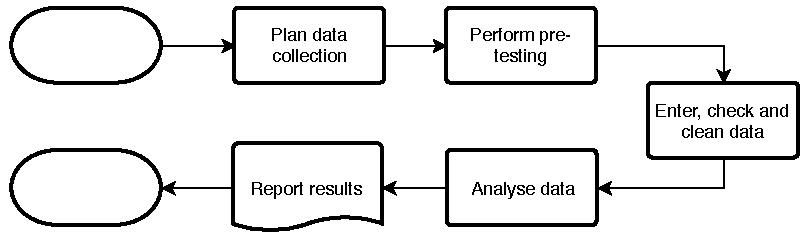
\includegraphics[width=0.9\linewidth]{gfx/standard/quesPretesting}} \quad
\caption[Questionnaire pre-testing process]{Questionnaire pre-testing process}\label{fig_quesPretesting}
\end{figure}

\subsubsection{Plan pre-testing}
Pre-testing a questionnaire requires researchers to plan well in advance to collect high-quality data. Planning a pre-testing involves deciding:

\begin{enumerate}
    \item \emph{Target respondents participation}: researchers shall decide if respondents participation is needed or available. If participants are needed, they shall represent target respondents \cite{Krosnick2009,Boynton2004}.
    Researchers shall use sampling techniques to select participants \cite{Boynton2004c,Diem,Radhakrishna2007}. They can find a set of techniques and details on how to use them online\footnote{Sampling techniques: \url{https://www.bmj.com/content/328/7451/1312?panels_ajax_tab_tab=jnl_bmj_tab_related_art&panels_ajax_tab_trigger=related\#d}}.
    Regarding the number of participants, researchers should prefer fewer answers with good quality, than a high number of answers with inaccurate or incomplete responses \cite{Boynton2004}. On the other hand, if respondents participation is not required, researchers shall invite experts to test and evaluate the questionnaire.
    
    \item \emph{Collection methods and procedures}: when researchers decide not to include respondents, pre-testing should be conducted using methods such as expert review, statistical modelling or \ac{AI} techniques. On the other hand, if target respondents participation is required, pre-testing should be conducted in similar conditions to a real questionnaire administering session \cite{Krosnick2009}. In that case, researchers shall choose the data collection method based on target respondents needs and preferences, which have been identified during the design stage. Also, researchers shall consider available resources and the evaluation goal \cite{Boynton2004}.
    Data collection methods include personal interviews, focus groups, mail questionnaires, web based questionnaires, telephone interviews, post questionnaires and interviewer guided \cite{Crawford1997,Diem,Boynton2004}. Researchers can find pros and cons of each method online\footnote{Data collection methods: \url{https://www.bmj.com/content/328/7452/1372?panels_ajax_tab_tab=jnl_bmj_tab_related_art&panels_ajax_tab_trigger=related\#3}}.
    Researchers shall be aware of data protection laws and internal codes, e.g., from researchers' or respondent's organisations \cite{Boynton2004}.
    
    \item \emph{Interviewers training}: people who conduct the pre-testing shall be trained or supervised. They should be prepared for answering and managing respondents' questions and unexpected reactions \cite{Boynton2004b}.
\end{enumerate}

\subsubsection{Perform pre-testing}
During pre-testing researchers should observe, record or take notes on important issues such as misunderstood, surprising or confusing questions, the time required by respondents to complete the questionnaire and respondents' reactions \cite{Boynton2004}. Researchers shall assure privacy, anonymity and non-threatening surroundings. Additionally, when interviewers are helping respondents to fill in the questionnaires, they should avoid inflexions on voices, facial expressions or gestures to avoid biases \cite{Boynton2004b}.
Finally, researchers should thank respondents for their participation \cite{Diem}.

\subsubsection{Enter, check and clean data}
Researchers shall enter, check and clean data to be analysed. They shall agree on and understand the tools to be used for this stage. This process should be carried out as soon as data is collected to avoid having to process a large amount of data \cite{Boynton2004}.

\subsubsection{Analyse data}
Researches shall select an analysis method based on the collected data \cite{Boynton2004,Diem}. A set of analysis methods are listed online\footnote{Analysis methods: \url{https://www.bmj.com/content/328/7452/1372?panels_ajax_tab_tab=jnl_bmj_tab_related_art&panels_ajax_tab_trigger=related\#4}}. At this stage, researchers shall establish the questionnaire reliability using measures such as Test-Retest or Internal Consistency Measures \cite{Radhakrishna2007,Diem}. Finally, they should establish questionnaire validity using a panel of experts or field test. Also, they should use readability tests like the Fog Index or Flesch Reading Ease \cite{Radhakrishna2007}.

\subsubsection{Report results}
Researchers shall filter relevant data to be reported \cite{Boynton2004,Diem} and how they will present the results. A set of recommendations about how to present data is presented in \cite{Boynton2004}. Researchers shall focus report on presenting and discussing the main findings. Also, they shall report reliability and validity indicating how these measures were established \cite{Radhakrishna2007}.

\subsection{Guide for formulating questions}
\label{sec:questions_guide}
When composing questionnaire questions, the following recommendations should be considered:

\begin{enumerate}
    \item Researchers should, if possible, involve representatives of target respondents in the design process of a questionnaire \cite{Boynton2004b}.
    
    \item Researchers should include explanations or examples when asking about abstract things \cite{Boynton2004b,Crawford1997}. However, specific and concrete wording is preferred over abstract wording \cite{Krosnick2009}.
    
    \item Researchers should use simple vocabulary that respondents can understand. They should consider that some words have different meanings in different contexts \cite{Boynton2004b,Diem,Krosnick2009}.
    
    \item Researchers should avoid complex routing for screening questions since that reduce respondents motivation and lead to indiscriminate answers \cite{Boynton2004b}.
    
    \item Researchers should pay careful attention to the demographic data that they intend to collect. They should avoid asking sensitive and threatening data. Pre-testing questionnaires allow identifying this issue \cite{Boynton2004b}.
    
    \item Researchers should, if possible, use official translators or translation services when developing questionnaires in more than one language \cite{Boynton2004b}.
    
    \item Researchers should avoid excluding disadvantaged groups of respondents to avoid biases, misunderstandings or ambiguity\cite{Boynton2004b}.
    
    \item Researchers should use specific adverbs instead of frequently, regularly, commonly, usually and hardly among others \cite{Boynton2004c,Krosnick2009}.
    
    \item Researchers should offer enough answer options when using closed questions to avoid respondents' frustration \cite{Boynton2004c}. Also, answer options should be mutually exclusive \cite{Krosnick2009}.
    
    \item Researchers should carefully plan when using open questions. They should consider time, skills and resources required for respondents to answer and for researchers to analyse the questionnaire \cite{Boynton2004c}.
    
    \item Researchers should avoid starting questionnaires with threatening questions \cite{Diem}.
    
    \item Researchers should include simple instructions \cite{Diem}.
    
    \item Researchers should be as brief as possible \cite{Diem}.
    
    \item Researchers should ask one question at a time \cite{Diem,Krosnick2009}.
    
    \item Researchers should include easy to answer questions at the beginning of a questionnaire \cite{Crawford1997,Krosnick2009}. Initial questions should also address the questionnaire topic directly \cite{Krosnick2009}.
    
    \item Researchers should order questions in a way that one leads naturally to the other. Additionally, researchers should be group questions on the same topic \cite{Crawford1997,Krosnick2009}.
    
    \item Researchers should include sensitive questions at the end of a questionnaire to avoid respondents cutting off before important information is collected \cite{Crawford1997,Krosnick2009}.
    
    \item Researchers should allow filtering questions to avoid that respondents answer questions that do not apply to them \cite{Krosnick2009}.
    
    \item Researchers should include a balanced number of answer options when using rating scales. Five to seven options have been proved to lead to reliable and valid questionnaires \cite{Krosnick2009}.
    
    \item Researchers should label points of rating scales. They should divide points into approximately equal units \cite{Krosnick2009}.
    
    \item Researchers should assure anonymity to avoid social desirability response bias \cite{Krosnick2009}.
    
    \item Researchers should avoid burdening respondents. To achieve this, they should reduce the reference period, use yes/no questions instead of all that apply questions and avoid making respondents perform computations that researchers can do \cite{Krosnick2009}.
\end{enumerate}

% -----------------------------------------------
\section{Validation} % Validation -----------------------------------------------
We started a submission process for our standard proposal at \ac{ICONTEC}, the Colombian Member Body of \ac{ISO} since it can submit a new work item proposal to the ISO/TC159/SC4 Ergonomics of human-system interaction technical committee. We have become a member of the Technical Committee 20 of \c{ICONTEC} (\textit{Comit\'e T\'ecnico de Normalizaci\'on (CTN) 20 Ergonom\'ia)}, we should participate in some meetings before they can consider our proposal for submission.

% -----------------------------------------------
%\section{Discussion} % Discussion -----------------------------------------------
%Reiterate the Research Problem/State the Major Findings: 
%Explain the Meaning of the Findings and Why They are Important: expected? unexpected? (explain these especially). unusual or unanticipated patterns or trends that emerged from your results and explain their meaning in relation to the research problem. 
%Relate the Findings to Similar Studies: compare your results with other studies or use the studies to support a claim.
%Consider Alternative Explanations of the Findings: a claim for how the results can be applied more generally. For example, describing lessons learned, proposing recommendations that can help improve a situation, or highlighting best practices.
%End: concise summary of the principal implications of the findings regardless of significance. Why you believe the findings and conclusions of your study are important and how they support broader knowledge or understanding of the research problem. This can be followed by any recommendations for further research. A more general claim or possible conclusion arising from the results. E.g. new research questions.

% -----------------------------------------------
\section{Conclusion} % Conclusion -----------------------------------------------
\label{sec:conclusion_2}
We presented a standard proposal for developing questionnaires to evaluate \ac{PX} aspects. Our proposal integrates practices that have been adopted to develop well-known \ac{UX} and \ac{PX} questionnaires and recommendations from questionnaire development experts. We identified the most influential standardisation organisation (i.e., \ac{ISO}) and its Colombian Body Member (\c{ICONTEC}) to start a submission process for our standard proposal. Our may contribution is related to standardising the process of developing reliable a valid questionnaires for evaluating \ac{PX} aspects, thereby making possible to compare and use results from different questionnaires uniformly.
